\chapter{总体设计}
\section{软件描述}
系统包括前台和后台两个部分。

前台主要功能是:初始化界面的显示、用户的登录相关操作的请求(如输入用户名密码等)、用户的文件相关操作的请求(如选中文件并上传、下载、分享等操作)的控制信息的发送以及数据文件的发送、用户操作的结果显示等。

后台主要功能是:处理用户的输入,判断其权限、其操作是否合法;对于相应的文件操作,进行相应的判断与处理,比如:对于上传以及分享的文件,进行内容审核处理;对文件进行存储冗余处理;并且将处理结果(包括操作的结果以及下载操作对应的数据文件的发送等)返回到客户端。

\section{处理流程}
\subsection{总体流程}
总体流程图如图3.1所示。总体上来说,客户端将用户的请求通过网络发送到服务器端,服务器端对该请求进行检查,审核等处理之后,再执行相关操作,并最终将操作的结果返回到客户端。
\begin{figure}[ht] 
\centering
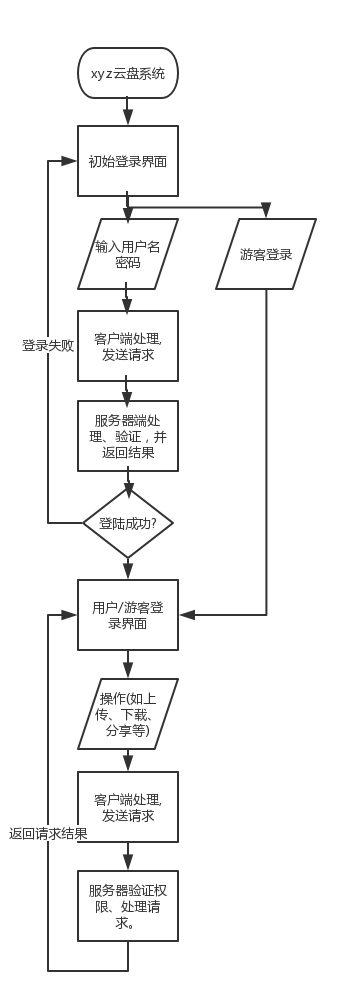
\includegraphics[width=7cm]{flow_overall.png} 
\caption{总体流程图}\label{fig:noted-figure}
\end{figure}

\subsection{系统基本流程}
系统基本流程如图3.2所示。
\begin{figure}
\centering
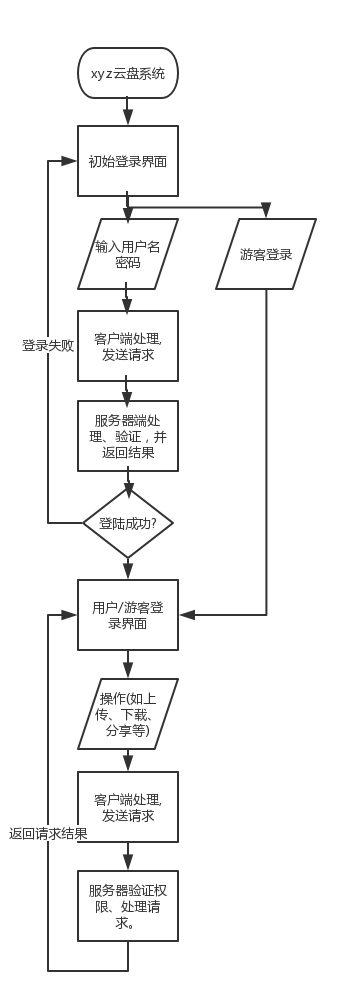
\includegraphics[width=7cm]{flow_system.png}
\caption{系统基本流程图}\label{fig:noted-figure}
\end{figure}

\subsection{客户端基本流程}
这只是举个例子,如果没有客户端则不需要此节。

\subsection{服务器端基本流程}
这只是举个例子,如果没有服务器端则不需要此节。

\subsection{功能1具体流程}
举个例子:交易处理流程

已登录用户在购物车中提交请求交易的 POST 请求,提交的表单中指明了交易中包括的
所有商品、商家、付款信息、收货地址,输入输出处理系统接收到合法请求后,向商品信息
系统请求数据,收到数据以后验证是否正确,然后向订单系统发起生成新订单的请求,订单
系统负责更新商品信息系统、商家信息,通知商家接单,返回订单处理结果输入输出处理系
统,输入输出处理系统依照结果产生 HTML 页面,并返回给用户。

\subsection{功能2具体流程}
此处应当有描述。

\subsection{功能3具体流程}
此处应当有一个描述。



\section{功能结构设计}
\subsection{整体结构}
此处应当有一个图和对应的描述。系统如果像微内核那样,划分成核心模块和若干个子系统,此处应当有图示及说明,然后后续几个节应当描述这几个子系统。如果系统像宏内核,那应当说明有哪些紧密联系的模块,并在后续几个节内描述这些模块。

\subsection{用户端结构}
此处应当有一个图和对应的描述。这只是举个例子。可能的内容包括用户端的具体模块、耦合情况等。

\subsection{服务器端结构}
此处应当有一个图和对应的描述。这只是举个例子。

\subsection{后台数据库维护模块结构}
此处应当有一个图和对应的描述。这只是举个例子。



\section{功能需求与程序代码的关系}
[此处指的是不同的需求分配到哪些模块去实现。可按不同的端拆分此表]
\begin{table}[htbp]
\centering
\caption{功能需求与程序代码的关系表} \label{tab:requirement-module}
\begin{tabular}{|c|c|c|c|}
    \hline
    · & 模块1 & 模块2 & 模块3 \\
    \hline
    需求1 & · & Y & · \\
    \hline
    需求2 & · & Y & · \\
    \hline
    需求3 & · & Y & · \\
    \hline
    需求4 & Y & · & · \\
    \hline
    需求5 & · & · & Y \\
    \hline
\end{tabular}
\note{各项功能需求的实现与各个程序模块的分配关系}
\end{table}